\section{Various Cuts}
The data used for calibration is from cosmic ray muons. These cosmic rays hit randomly throughout the PCAL unit. 
The distribution of these events although expected to be uniform, don't guarantee a good hit or detected signal in all three layers.
Moreover due to the strange pixel shapes and varying sizes different pixels have very different number of counts. 
An intitial skim was used to cut out events that would prevent a clean signal for calibration purposes.
Events were removed based on a multiplicity cut and a Dalitz condition.



\FloatBarrier
\subsection{Multiplicity Cut}
To ensure a more accurate calibration, a multiplicity cut was applied to the collected data. 
The multiplicity cut removed any event that contained more than three PMT readouts (one in each layer). 
This reduces the number of cosmic ray events that are not relatively perpendicular to the face of the PCAL unit.
This is due to the fact that if a cosmic ray trajectory is not perpendicular to the PCAL face, it could clip multiple strips 
in one orientation (i.e. strip U30 and U31 both recieve a signal). Therefore, by restricting the calibration to one perpendicular
hit, more well defined calibration constants could be determined. The accepted range of angles (different from perpendicular
to the PCAL face) varies as a function of strip number and is not uniform in all directions. This multiplicity cut also 
helps in removing events where multiple cosmic rays hit the detector within the same time interval, due to possible firing of more PMTs. 



 \FloatBarrier
\subsection{Dalitz Cut} 
The Dalitz condition implies that if a point inside a triangle is chosen, no matter the location, the sum of the distances to each edge will be unchanged.
Rather than calculating each x and y point for every hit, distance as a function of strip width can be used to test this condition.
The relatively simple strip calculation can be computed by knowing the corresponding strip number to the triggered PMT combined with equations \ref{eq:udist}-\ref{eq:totaldist}.
This distance is empirically found to be two.
Preskimmed data demonstrating this distribution can be found at \url{https://clasweb.jlab.org/wiki/index.php/PCAL_Cosmic_Ray_Tests}. 
If this condition is not satisfied, then the hit recorded is most likely electronic noise, an indirect hit, or multiple cosmic ray hits recorded at once.

\begin{equation}
    dist(u) = \left\{
        \begin{array}{l l}
            u/84.0                       & \quad \text{if $u < 52$}\\
            (52.0 + (u - 52.0)\times2.0)/84.0 & \quad \text{if $u \geq 52$}
        \end{array} \right.{}
         \label{eq:udist}
\end{equation}

\begin{equation}
    dist(v) = \left\{
        \begin{array}{l l}
            2.0 \times v/77.0;                       & \quad \text{if $v < 15$}\\
            (30.0 + (v - 15.0))/77.0                 & \quad \text{if $v \geq 15$}
        \end{array} \right.{}
         \label{eq:vdist}
\end{equation}


\begin{equation}
    dist(w) = \left\{
        \begin{array}{l l}
            2.0 \times w/77.0;                       & \quad \text{if $w < 15$}\\
            (30.0 + (w - 15.0))/77.0                 & \quad \text{if $w \geq 15$}
        \end{array} \right.{}
         \label{eq:wdist}
\end{equation}


\begin{equation} 
    uvw = dist(u) +  dist(v) + dist(w)
    \label{eq:totaldist}
\end{equation}

\begin{figure}[h]
    \centering
    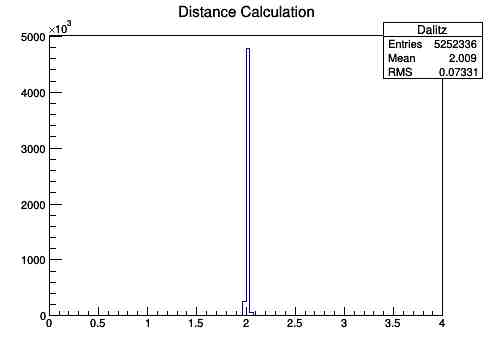
\includegraphics[height= 3in, keepaspectratio = true]{dalitz}
    \caption{Plotted is the resulting number ($uvw$) obtained from equation \ref{eq:totaldist} after the initial skim.}
    \label{fig:dalitz}
\end{figure} 


\FloatBarrier
\subsection{Unphysical Events}
\label{sec:unphysical}
An investigation into the types background was performed. 
Looking at an occupation number (events within a pixel), some recorded hits were unphysical if only one cosmic ray was considered to prompt the signal. 
Examples can be seen by Figures \ref{fig:unphysical} and \ref{fig:occupationnum}.

\begin{figure}[h]
    \centering
    \begin{subfigure}[h]{0.44\textwidth}
        \centering
        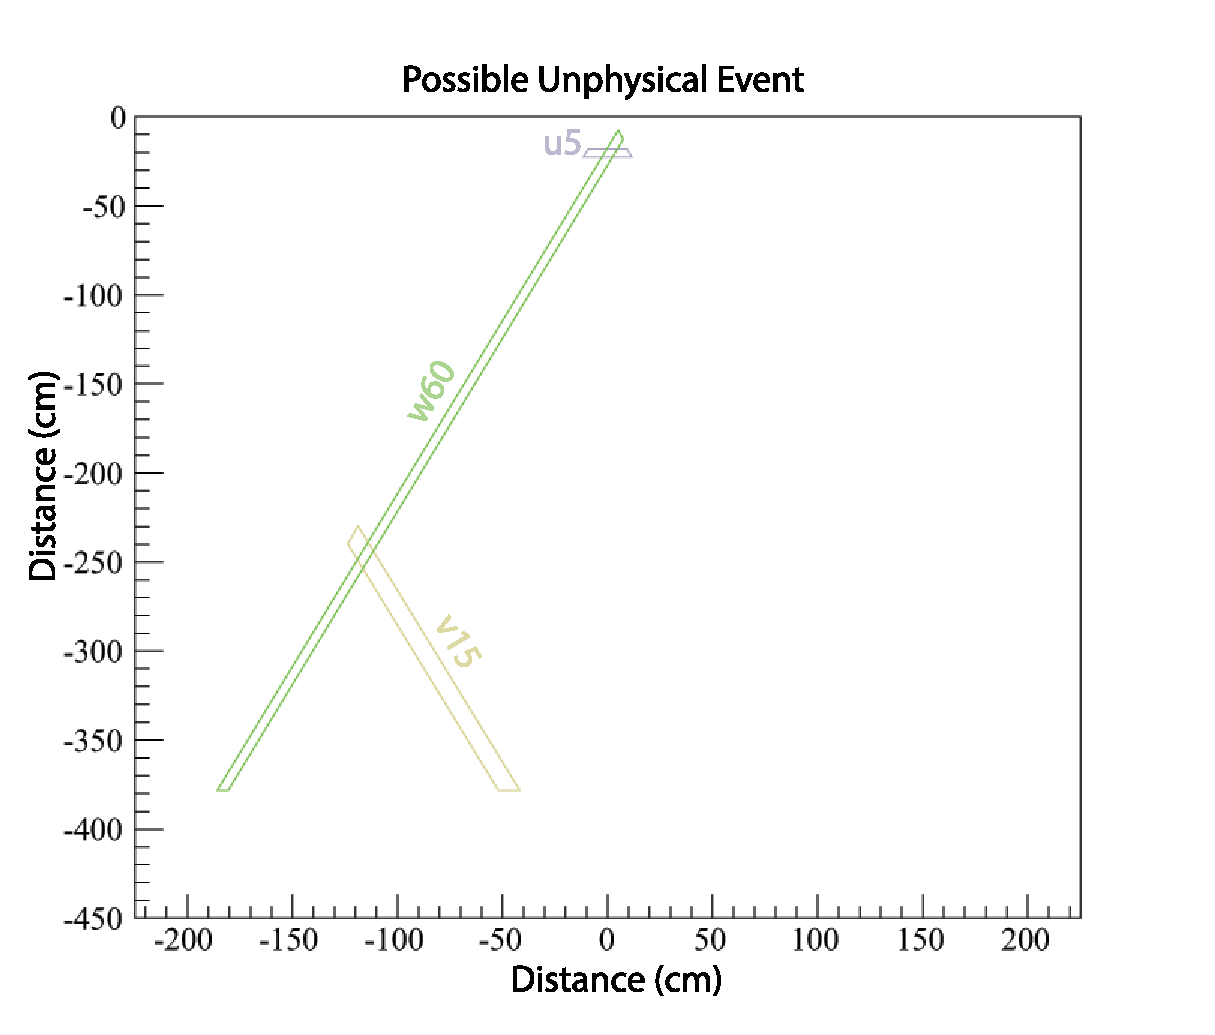
\includegraphics[width=\textwidth, keepaspectratio = true]{unphysical}
        \caption{Shown is one example of an event that would pass a multiplicity cut, but is clearly from either multiple rays or other noise.}
        \label{fig:unphysical}
    \end{subfigure}
    ~
    \begin{subfigure}[h]{0.44\textwidth}
        \centering
        \includegraphics[width=\textwidth, keepaspectratio = true]{pixelmap}
        \caption{Shown is a rough outline of the scintillator mapping created with minimal input.}
        \label{fig:pixelmap}
    \end{subfigure}
    \caption{Rough outline of the PCAL system.}
    \label{fig:pixelexplain}
\end{figure}

\begin{figure}[h]
\centering
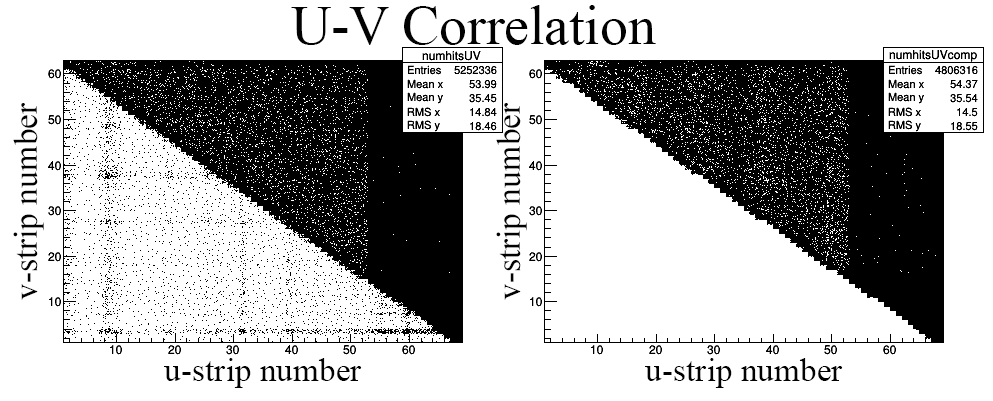
\includegraphics[width= 6in, keepaspectratio = true]{occupationnum}
\caption{The left histogram shows the U and V strip correlation after both the multiplicity and dalitz cuts were applied. The right 
histogram shows the U and V strip correlation after rejecting all known unphysical background.}
\label{fig:occupationnum}
\end{figure}


Some of the unphysical events can be spotted easily because low u and low v strip numbers should never correlate to just one incident cosmic ray.
To investigate in more detail, a program outlining the PCAL detector by strip number was generated.
This was generated using $\alpha$, $\beta$, number of strips, and strip width ($w$) as defined by Figure \ref{fig:stripwidth}. This outline or pixel mapping can be seen in Figure \ref{fig:pixelmap}.
This ideal outline of the system was then used in combination with a random number generator to verify which strip numbers could correlate to a physical perpendicular trajectory through the system.
These correlation numbers were then stored in tables and recalled in the analysis. Neighboring pixels in all directions were also marked as valid to account for uncertainty in the calculations and given numbers. 
Removing any event that did not end up in correlated PMTs results in no obvious unphysical signals as seen in figure \ref{fig:occupationnum}. 
However, looking at the signal distribution an exponential background still appears. This demonstrates that either different cuts and/or a very good fitting routine needs to be put in place.



\FloatBarrier
